\documentclass[11pt]{article}

% Setting up the page
\usepackage[english]{babel}
\usepackage[utf8]{inputenc}
\usepackage{fullpage}

% Bibliography
\usepackage[numbers]{natbib}
\bibliographystyle{spmpsci}

% Writing mathematics, algorithms and code
\usepackage{amsmath}
\usepackage{amssymb}
\usepackage{amsthm}
    \newtheorem{definition}{Definition}
    \newtheorem{theorem}{Theorem}
\usepackage{mathtools} % lvert and rvert
    \DeclarePairedDelimiter\abs{\lvert}{\rvert}%
    \DeclarePairedDelimiter\norm{\lVert}{\rVert}%
\usepackage[boxruled]{algorithm2e}
    \newcommand{\balg}{\begin{algorithm}[htbp]\DontPrintSemicolon}
    \newcommand{\ealg}{\end{algorithm}}

% Images, tables and referencing
\usepackage{booktabs}
\usepackage{caption, subcaption}
    \captionsetup[figure]{name={Figure}, labelsep=colon}
\usepackage{graphicx}
\usepackage{hyperref}

\newcommand{\imgwidth}{.85\textwidth}
\newlength{\tablewidth}
\setlength{\tablewidth}{.9\textwidth}

\title{%
    A novel initialisation based on hospital-resident assignment for the
    \(k\)-modes algorithm
}
\author{Henry Wilde, Vincent Knight and Jonathan Gillard}

\begin{document}

\maketitle%
\begin{abstract}
    This paper presents a new way of selecting an initial solution for the
    \(k\)-modes algorithm that allows for a notion of game theoretic fairness
    that classic initialisations, namely those by Huang and Cao, do not. The
    method, which utilises the Hospital-Resident Assignment Problem to find the
    set of initial cluster centroids, is compared with two initialisation
    methods for \(k\)-modes~\cite{Huang1998} as well as the next most popular
    method present in the literature~\cite{Cao2009}. In order to highlight the
    merits of the proposed method two stages of analysis are presented. The
    paper concludes with an analysis of these methods against the proposed and
    it is demonstrated that the proposed method is able to outperform them both.
    The aim of this analysis is two-fold: first, to highlight the merits of the
    method in a familiar setting by clustering well-known benchmark datasets;
    and second, to provide a deeper insight into how the methods perform against
    one another by generating artificial datasets using the method set out
    in~\cite{Wilde2019}.
\end{abstract}

\section{Introduction}\label{sec:intro}

Clustering is an unsupervised learning technique for discovering intrinsic
structure within data. There exist many approaches to clustering but perhaps the
most ubiquitous amongst them is centroid-based clustering. This approach aims to
maximise summed within-cluster similarity by iterating over the points in a
dataset and adjusting the current clusters according to some measure for central
tendency until convergence. A popular algorithm for performing centroid-based
clustering is the \(k\)-means algorithm. In \(k\)-means, a number of groups to
identify in a dataset, \(k\), is fixed \emph{a priori} and each cluster has
associated with it a centroid or representative point calculated as the mean of
the data points within that cluster. Unfortunately, this is only valid for
numeric data where the mean of a set is well-defined. Despite this, the paradigm
in which \(k\)-means clustering exists is of interest as it is fast, scalable,
easily parallelised, and simple in its design~\cite{Wu2009,Zhao2009}.

In this work, the focus will be on \(k\)-modes clustering; an extension to
\(k\)-means that permits the sensible clustering of categorical (i.e.\ ordinal,
nominal or otherwise discrete) data as set out in the seminal works by
Huang~\cite{Huang1997a,Huang1997b,Huang1998}. An alternative, though largely
equivalent, form for \(k\)-modes was presented in~\cite{Chaturvedi2001} but is
not considered in this work. Under this framework, the central tendency measure
used is the mode and Euclidean distance is replaced by a simple matching
measure. All of the concepts used to define the \(k\)-modes algorithm are
presented later in this section.

The interest of this paper is in how the performance of the \(k\)-modes
algorithm may be affected. Since the \(k\)-modes algorithm is a heuristic, its
performance is dependent on its initial solution. The quality of the initial
solution is affected by two components: the metric being used and the process by
which the solution is chosen.

Strictly, introducing a new metric alters the space in which the data exists and
its effect on the initial solution is not independent of the final solution.
Having said that, following the seminal \(k\)-modes papers, a number of
alternative dissimilarity measures have been implemented to improve on the
simple matching dissimilarity used most regularly. The main drawback of the
standard measure is that it often produces clusters with low intra-cluster
similarity~\cite{Ng2007} and does not take into account any relationships
between attributes or their categories. Other measures have been designed to be
used in a specific context where such relationships may be
considered~\cite{Cao2012,Yu2018,Zhou2016}. However, these measures sometimes are
defined between a point in the dataset and a centroid rather than defining a
metric for the entire space.

Instead of adjusting the overall space, this work considers the process by which
an initial solution is found. The proposed method is an extension to that
presented by Huang~\cite{Huang1998} that generates a game-theoretically fair and
stable variant to that generated by Huang's method. The remainder of this paper
is structured as follows:
\begin{itemize}
    \item Section~\ref{sec:intro} introduces the \(k\)-modes algorithm and its
        established initialisation methods.
    \item Section~\ref{sec:method} provides a brief overview of
        matching games and their variants before a statement of the proposed
        initialisation method.
    \item Section~\ref{sec:results} presents analyses of the initialisation
        methods on benchmark and new, artificial datasets.
    \item Section~\ref{sec:conclusion} concludes the paper.
\end{itemize}


\subsection{The \(k\)-modes algorithm}\label{subsec:kmodes}

The following notation will be used throughout this work to describe the objects
associated with clustering a dataset:

\begin{itemize}
    \item Let \(\mathcal{A} := A_1 \times \cdots \times A_m\) denote the
        \emph{attribute~space}. In this work, only categorical attributes are
        considered and so it is intuitive to describe each attribute as a set of
        its values, i.e.\ for each \(j = 1, \ldots, m\) it follows that \(A_j :=
        \left\{a_1^{(j)}, \ldots, a_{d_j}^{(j)}\right\}\) where \(d_j = |A_j|\)
        is considered the size of the \(j^{th}\) attribute.

    \item Let \(\mathcal{X} := \left\{X^{(1)}, \ldots, X^{(N)}\right\} \subset
        \mathcal{A}\) denote a \emph{dataset} where each \(X^{(i)} \in
        \mathcal{X}\) is defined as an \(m\)-tuple \(X^{(i)} := \left(x_1^{(i)},
        \ldots, x_m^{(i)}\right)\) where \(x_j^{(i)} \in A_j\) for each \(j = 1,
        \ldots, m\). The elements of \(\mathcal{X}\) are referred to as
        \emph{data points} or \emph{instances}.
%        A dataset \(\mathcal{X}\) can be
%        represented as a table like so:
%        \begin{table}[H]
%        \centering
%        \begin{tabular}{cccccc}
%            {} & \(A_1\) & \(A_2\) & \quad \ldots \quad & \(A_{m-1}\) & \(A_m\)
%            \\
%            \midrule
%            \(X^{(1)}\) & \(x_1^{(1)}\) & \(x_2^{(1)}\) & \quad \ldots \quad & 
%            \(x_{m-1}^{(1)}\) & \(x_m^{(1)}\)
%            \\
%            \(X^{(2)}\) & \(x_1^{(2)}\) & \(x_2^{(2)}\) & \quad \ldots \quad &
%            \(x_{m-1}^{(2)}\) & \(x_m^{(2)}\)
%            \\
%            \vdots & \vdots & \vdots & {} & \vdots & \vdots
%            \\
%            \(X^{(N)}\) & \(x_1^{(N)}\) & \(x_2^{(N)}\) & \quad \ldots \quad &
%            \(x_{m-1}^{(N)}\) & \(x_m^{(N)}\)
%        \end{tabular}
%        \end{table}

    \item Let \(\mathcal{Z} := \left(Z_1, \ldots, Z_k\right)\) be a partition
        of a dataset \(\mathcal{X}\) into \(k \in \mathbb{Z}^{+}\) distinct,
        non-empty parts. Such a partition \(\mathcal{Z}\) is called a
        \emph{clustering} of \(\mathcal{X}\).

    \item Each cluster \(Z_l\) has associated with it a
        \emph{representative~point} (see Definition~\ref{def:mode}) which is
        denoted by \(z^{(l)} = \left(z_1^{(l)},~\ldots,~z_m^{(l)}\right) \in
        \mathcal{A}\).  These points may also be referred to as cluster modes.
        The set of all current representative points is denoted \(\overline Z =
        \left\{z^{(1)}, \ldots, z^{(k)}\right\}\).
\end{itemize}

As is discussed above, the notion of distance is lost in categorical space, and
especially when that space is even partly nominal. Definition~\ref{def:dissim}
describes a simple dissimilarity measure between categorical data points.

\begin{definition}\label{def:dissim}
    Let \(\mathcal{X}\) be a dataset and consider any \(X^{(a)}, X^{(b)} \in
    \mathcal{X}\). The dissimilarity between \(X^{(a)}\) and \(X^{(b)}\),
    denoted by \(d\left(X^{(a)}, X^{(b)}\right)\), is given by:
    \begin{equation}\label{eq:dissim}
        d\left(X^{(a)}, X^{(b)}\right) := \sum_{j=1}^{m} \delta\left(x_j^{(a)},
        x_j^{(b)}\right) \quad \text{where} \quad \delta\left(x, y\right) =
        \begin{cases}
            0, & \text{if} \ x = y \\
            1, & \text{otherwise.}
        \end{cases}
    \end{equation}
    In other words, the dissimilarity between two points is the number of
    attributes where their values are not the same. A proof
    that~\eqref{eq:dissim} is a valid distance metric is given as an appendix.
\end{definition}

%\begin{example}\label{ex:dissim}
    Throughout this work, we will make use of a number of small examples to aid
    our understanding of various concepts. These examples will utilise a small,
    artificial dataset describing some qualities about vehicles.
    
    The dataset is made up of \(N = 10\) instances, each of which describe a
    vehicle. These instances are defined by \(m = 6\) attributes, the first two
    of which are ordinal variables taken from the set \(\{\text{L, M, H, V}\}\)
    standing for `low', `medium', `high', and `very high' respectively. The
    next three are integer variables and so can be considered as categorical,
    and the final attribute is a binary variable indicating whether the vehicle
    is eco-friendly \((1)\) or not \((0)\). The full dataset is given in
    Table~\ref{tab:dataset}. Please note that there is an additional, unheaded
    column on the left hand side showing the index starting at \(1\) and going
    up to \(5\).
    
    \begin{table}[H]
        \centering
        \singlespacing{%
        \resizebox{.8\textwidth}{!}{%
            \centering
            \begin{tabular}{lllrrrr}
\toprule
{} & Price & Maintenance &  Doors &  Passengers &  Wheels &  Eco-Friendly \\
\midrule
0 &     H &           M &      2 &           2 &       4 &             0 \\
1 &     L &           M &      0 &           1 &       2 &             0 \\
2 &     V &           H &      2 &           3 &       8 &             0 \\
3 &     H &           L &      4 &           5 &       4 &             1 \\
4 &     M &           M &      2 &           5 &       4 &             1 \\
5 &     M &           L &      2 &           4 &       4 &             1 \\
6 &     V &           H &      4 &           5 &       4 &             0 \\
7 &     L &           V &      2 &           4 &       4 &             0 \\
8 &     H &           M &      0 &           2 &       2 &             1 \\
9 &     H &           M &      4 &           7 &       4 &             0 \\
\bottomrule
\end{tabular}

        }}
        \caption{The vehicle dataset.}\label{tab:dataset}
    \end{table}

    Let us consider our first two datapoints. With the notation laid out in
    Section~\ref{subsec:notation}, we can express these points as vectors in the
    following way:

    \begin{equation}
        \nonumber
        \begin{aligned}
            X^{(1)} & = & \left[ x_1^{(1)} = \text{H}, \ x_2^{(1)} = \text{M}, \
            x_3^{(1)} = 2, \ x_4^{(1)} = 2, \ x_5^{(1)} = 4, \ x_6^{(1)} = 0 
            \right]
            \\
            X^{(2)} & = & \left[ x_1^{(2)} = \text{L}, \ x_2^{(2)} = \text{M}, \
            x_3^{(2)} = 0, \ x_4^{(2)} = 1, \ x_5^{(2)} = 2, \ x_6^{(2)} = 0
            \right]
        \end{aligned}
    \end{equation}

    Then, by Definition~\ref{def:dissim}, their pairwise dissimilarity is:
    \begin{equation}
        \nonumber
        \begin{aligned}
            \centering
            d(X^{(1)}, X^{(2)}) & = & \delta(\text{H}, \text{L}) & + & 
            \delta(\text{M}, \text{M}) & + & \delta(3, 0) & + & \delta(2, 1) &
            + & \delta(4, 2) & + & \delta(0, 0) & {} & {}
            \\
            {} & = & 1 \ & + & 0 \ & + & 1 \ & + & 1 \ & + & 1 \ & + & 0 \ & = &
            4
        \end{aligned}
    \end{equation}
\end{example}


With this metric defined, the notion of a representative point within a cluster
can be addressed. When clustering numeric data, a centroid of a cluster is taken
to be the average of the points within the cluster so as to summarise the
information contained within that cluster. With categorical data, however, a
frequency approach is used. This follows from the concept of dissimilarity
where the point that best represents (i.e.\ is closest to) those in a cluster
is one with the most frequent attribute values of the points in the cluster. As
such, a representative point of a cluster is often called a mode. The following
definitions and theorem formally define such a representative point and a means
of finding them.

\begin{definition}\label{def:mode}
    Let \(\mathcal{X} \subset \mathcal{A}\) be a dataset and consider some point
    \(z = \left(z_1, \ldots, z_m\right) \in \mathcal{A}\). Then \(z\) is called
    a \emph{mode} of \(\mathcal{X}\) if it minimises the following:
    \begin{equation}\label{eq:summed-dissim}
        D\left(\mathcal{X}, z\right) = \sum_{i=1}^{N} d\left(X^{(i)}, z\right)
    \end{equation}
\end{definition}

\begin{definition}\label{def:rel-freq}
    Let \(\mathcal{X} \subset \mathcal{A}\) be a dataset. Then
    \(n\left(a_s^{(j)}\right)\) denotes the \emph{frequency} of the \(s^{th}\)
    category \(a_s^{(j)}\) of \(A_j\) in \(\mathcal{X}\), i.e.\ for each \(A_j
    \in \mathcal{A}\) and each \(s = 1, \ldots, d_j\):
    \begin{equation}
        n\left(a_s^{(j)}\right) := \abs*{%
            {\left\{X^{(i)} \in \mathcal{X}: x_j^{(i)} = a_s^{(j)}\right\}}
        }
    \end{equation}
	
    Furthermore, \(\frac{n\left(a_s^{(j)}\right)}{N}\) is called the
    \emph{relative~frequency} of category \(a_s^{(j)}\) in \(\mathcal{X}\).
\end{definition}

\begin{theorem}\label{thm:mode}
    Consider a dataset \(\mathcal{X} \subset \mathcal{A}\) and some \(U = (u_1,
    \ldots, u_m) \in \mathcal{A}\). Then \(D(\mathcal{X}, U)\) is minimised if
    and only if \(n\left(u_j\right) \geq n\left(a_s^{(j)}\right)\) for all
    \(s=1, \ldots, d_j\) for each \(j = 1, \ldots, m\).

    A proof of this theorem can be found in the Appendix of~\cite{Huang1998}.
\end{theorem}

%\begin{example}\label{ex:mode}
    Let us return to our vehicale dataset from Example~\ref{ex:dissim}. Using 
    Theorem~\ref{thm:1}, we can identify a mode of our set by taking the most 
    commonly occurring value for each attribute. We can then take these values
    as a vector and call it \(\mu\). In this case, we have:

    \[ 
 	 \mu = \left[\text{H}, \ \text{M}, \ \text{2}, \ \text{5}, \ \text{4}, \ \text{0}\right] 
\]

    This point actually appears in our dataset and corresponds to the first row.
    It is easily verified (a Python script doing so is given as an Appendix)
    that this point is in fact the only point in the span of the attribute space
    \(A_1 \times \cdots \times A_6\) that minimises our summed dissimilarity. In
    this way, we have that the first row of our dataset is the only true mode of
    our set, virtual or not.
\end{example}



Theorem~\ref{thm:mode} defines the process by which representatives are updated
in \(k\)-modes (see Algorithm~\ref{alg:update}), and so the final component from
the \(k\)-means paradigm to be configured is the objective (cost) function. This
function is defined in Definition~\ref{def:cost}, and following that a practical
statement of the \(k\)-modes algorithm is given in Algorithm~\ref{alg:kmodes} as
set out in~\cite{Huang1998}.

\begin{definition}\label{def:cost}
    Let \(\mathcal{Z} = \left\{Z_1, \ldots, Z_k\right\}\) be a clustering of a
    dataset \(\mathcal{X}\), and let \(\overline Z = \left\{z^{(1)},
    \ldots, z^{(k)}\right\}\) be the corresponding cluster modes. Then \(W =
    \left(w_{i, l}\right)\) is an \(N \times k\) \emph{partition~matrix} of
    \(\mathcal{X}\) such that:
    \[
        w_{i, l} = \begin{cases}
                     1, & \text{if} \ X^{(i)} \in Z_l\\
                     0, & \text{otherwise.}
                   \end{cases}
    \]

    With this, the \emph{cost~function} is defined to be the summed
    within-cluster dissimilarity:
    \begin{equation}\label{eq:cost}
        C\left(W, \overline Z\right) := \sum_{l=1}^{k} \sum_{i=1}^{N}
        \sum_{j=1}^{m} w_{i,l} \ \delta\left(x_j^{(i)}, z_j^{(l)}\right)
    \end{equation}
\end{definition}

\begin{algorithm}[H]
    \caption{\(k\)-modes}\label{alg:kmodes}
	\begin{algorithmic}[0]
        \State{\textbf{Input:} a dataset \textbf{X}, a number of clusters to
        form \(k\)}
        \State{\textbf{Output:} a clustering of the dataset \(C_1, \ldots, 
        C_k\)\\}
        \\
        \Comment{Initialisation step}
        \State{\(\bar{\mu} \gets \emptyset\)}
        \For{\(l \in \{1, \ldots, k\}\)}
            \State{\(C_l \gets \emptyset\)}
		\EndFor
        \State{Select \(k\) initial modes, \(\mu^{(1)}, \ldots, \mu^{(k)} \in
        \textbf{X}\).}
        \State{\(\bar{\mu} \gets \left\{\mu^{(1)}, \ldots, 
            \mu^{(k)}\right\}\)\\}
        \\
        \Comment{First cluster assignment}
        \For{\(X_i \in \textbf{X}\)}
            \State{Select \(l^*\) that satisfies: 
                \[
                    d(X^{(i)}, \mu^{(l^*)}) = \min_{1 \le l \le m} 
                    \left\{d(X^{(i)}, \mu^{(l)})\right\}
                \]
            }
            \State{\(C_{l^*} \gets C_{l^*} \cup \{X^{(i)}\}\)}
            \State{\textsc{Update}\((\mu^{(l^*)})\).}
		\EndFor
        \\
        \\
        \Comment{Continue to reassign poiunts to the most similar cluster until
        no point moves}
        \Repeat{%
            \For{\(X^{(i)} \in \textbf{X}\)}
                \For{\(\mu^{(l)} \in \bar{\mu}\)}
                    \State{Calculate \(d(X^{(i)}, \mu^{(l)})\)}
				\EndFor
                \If{\(d(X^{(i)}, \mu^{(l^*)}) > d(X^{(i)}, \mu^{(l')}) \ 
                \text{for some} \ l' \neq l^*\)}
                    \State{\(C_{l^*} \gets C_{l^*} \setminus \{X^{(i)}\}\)}
                    \State{\(C_{l'} \gets C_{l'} \cup \{X^{(i)}\}\)}
                    \State{\textsc{Update}\((\mu^{(l^*)})\) and 
                    \textsc{Update}\((\mu^{(l')})\).}
				\EndIf
			\EndFor
        }
		\Until{No point changes cluster after a full cycle through \textbf{X}.}
	\end{algorithmic}
\end{algorithm}


The standard selection method to initialise \(k\)-modes is to randomly sample
\(k\) distinct points in the dataset. In all cases, the initial modes must be
points in the dataset to ensure that there are no empty clusters in the first
iteration of the algorithm. The remainder of this section describes two
well-established initialisation methods that aim to preemptively lever the
structure of the data at hand.


\subsection{Initialisation processes}\label{subsec:inits}

\subsubsection{Huang's method}\label{subsec:huang}

Amongst the original works by Huang, an alternative initialisation method was
presented that selects modes by distributing frequently occurring values from the
attribute space among \(k\) potential modes~\cite{Huang1998}. The process,
denoted as Huang's method, is described in full in Algorithm~\ref{alg:huang}.
Huang's method considers a set of potential modes,
\(\widehat Z \subset \mathcal A\), that is then replaced by the actual set of
initial modes, \(\overline Z \subset \mathcal X\).

In the original statement of Huang's method, it is stated that the most
frequent categories should be assigned `equally' to the set of potential modes.
How the categories should be distributed `equally' is not well-defined or easily
seen from the example given in the paper. In software implementations, including
the one used in Section~\ref{sec:results}, the term is taken to mean using a
probability distribution to sample values from the attribute space. This
probability distribution is formed by the relative frequencies of each
attribute's categories.

\balg%
    \caption{Huang's method}\label{alg:huang}
    \KwIn{a dataset \(\mathcal{X} \subset \mathcal{A}\), a number of modes to
    find \(k\)}
    \KwOut{a set of \(k\) initial modes \(\overline Z\)}

    \(\widehat Z \gets \emptyset\)\;
    \(\overline Z \gets \emptyset\)\;
    \For{\(j = 1, \ldots, m\)}{%
        \For{\(s = 1, \ldots, d_j\)}{%
            Calculate \(\frac{n(a_s^{(j)})}{N}\)
        }
    }

    \For{\(l = 1, \ldots, k\)}{%
        Create an empty \(m\)-tuple \(\hat{z}^{(l)}\)\;
        \For{\(j = 1, \ldots, m\)}{%
            Sample \(a_{s^*}^{(j)}\) from \(A_j\) with respect to the 
            relative frequencies of \(A_j\)\;
            \(\hat{z}_j^{(l)} \gets a_{s^*}^{(j)}\)
        }

        \(\widehat Z \gets \widehat Z \cup \left\{\hat{z}^{(l)}\right\}\)
    }

    \For{\(\hat{z} \in \widehat Z\)}{%
        Select \(X^{(i^*)} \in \mathcal{X}\) that satisfies: 
        \[
            \min_{1 \leq i \leq N} \left\{d\left(X^{(i)}, \hat{z}\right) \ | \
            X^{(i^*)} \notin \overline Z\right\}
        \]

        \(\overline Z \gets \overline Z \cup \left\{X^{(i^*)}\right\}\)
    }
\ealg%

%\balg%
    \caption{Huang's method}\label{alg:huang}
    \KwIn{a dataset \(\mathcal{X} \subset \mathcal{A}\), a number of modes to
    find \(k\)}
    \KwOut{a set of \(k\) initial modes \(\overline Z\)}

    \(\widehat Z \gets \emptyset\)\;
    \(\overline Z \gets \emptyset\)\;
    \For{\(j = 1, \ldots, m\)}{%
        \For{\(s = 1, \ldots, d_j\)}{%
            Calculate \(\frac{n(a_s^{(j)})}{N}\)
        }
    }

    \For{\(l = 1, \ldots, k\)}{%
        Create an empty \(m\)-tuple \(\hat{z}^{(l)}\)\;
        \For{\(j = 1, \ldots, m\)}{%
            Sample \(a_{s^*}^{(j)}\) from \(A_j\) with respect to the 
            relative frequencies of \(A_j\)\;
            \(\hat{z}_j^{(l)} \gets a_{s^*}^{(j)}\)
        }

        \(\widehat Z \gets \widehat Z \cup \left\{\hat{z}^{(l)}\right\}\)
    }

    \For{\(\hat{z} \in \widehat Z\)}{%
        Select \(X^{(i^*)} \in \mathcal{X}\) that satisfies: 
        \[
            \min_{1 \leq i \leq N} \left\{d\left(X^{(i)}, \hat{z}\right) \ | \
            X^{(i^*)} \notin \overline Z\right\}
        \]

        \(\overline Z \gets \overline Z \cup \left\{X^{(i^*)}\right\}\)
    }
\ealg%



\subsubsection{Cao's method}\label{subsec:cao}

The second initialisation process that is widely used with \(k\)-modes is known
as Cao's method~\cite{Cao2009}. This method selects representative points
according to their density in the dataset whilst forcing dissimilarity between
them. Definition~\ref{def:density} formalises the concept of density and its
relationship to relative frequency. The method, which is described in
Algorithm~\ref{alg:cao}, is often considered to be deterministic as there is no
formally stochastic element. However, this is only true up to an arbitrary
breaking of ties in the density-dissimilarity calculations and so many practical
implementations cannot guarantee a unique solution across multiple runs using
this method.

\begin{definition}\label{def:density}	
    Consider a data set \(\mathcal{X}\) with attribute set \(\mathcal{A} = 
    \{A_1, \ldots, A_m\}\). Then the \emph{average~density} of any point 
    \(X_i \in \mathcal{X}\) with respect to \(\mathcal{A}\) is 
    defined~\cite{Cao2009} as:
    \begin{equation}\label{eq:density}
        \text{Dens}\left(X^{(i)}\right) = \frac{%
            \sum_{j=1}^m \text{Dens}_{j}\left(X^{(i)}\right)
        }{m}
        \ \ \text{where} \ \
        \text{Dens}_{j}\left(X^{(i)}\right) = \frac{%
            \abs*{%
                \left\{X^{(t)} \in \mathcal{X} : x_j^{(i)} = x_j^{(t)}\right\}
            }
        }{N}
    \end{equation}

    Observe that:
    \[
        \abs*{\left\{X^{(t)} \in \mathcal{X} : x_j^{(i)} = x_j^{(t)}\right\}}%
        = n\left(x_j^{(i)}\right)%
        = \sum_{t=1}^N \left(1 - \delta\left(x_j^{(i)}, x_j^{(t)}\right)\right)
    \]

    And so, an alternative definition for~\eqref{eq:density} can be derived:
    \begin{equation}\label{eq:density-alt}
    \begin{aligned}
        \text{Dens}\left(X^{(i)}\right)
        & = \frac{1}{mN} \sum_{j=1}^m \sum_{t=1}^N \left(%
            1 - \delta\left(x_j^{(i)}, x_j^{(t)}\right)
        \right)\\
        & = \frac{1}{mN} \sum_{j=1}^m \sum_{t=1}^N 1%
            - \frac{1}{mN} \sum_{j=1}^m \sum_{t=1}^N
            \delta\left(x_j^{(i)}, x_j^{(t)}\right)\\
        & = \frac{mN}{mN} - \frac{1}{mN} \sum_{t=1}^N
            d\left(X^{(i)}, X^{(t)}\right)\\
        & = 1 - \frac{1}{mN} D\left(\mathcal{X}, X^{(i)}\right)
    \end{aligned}
    \end{equation}

    With this alternative definition, it is clear --- since \(m\) and \(N\) are
    fixed positive integers --- that \(\text{Dens}(X^{(i)})\) is maximised when
    \(D(\mathcal{X}, X^{(i)})\) is minimised. Then by Theorem~\ref{thm:mode},
    any data point with maximal average density is, in fact, a mode of
    \(\mathcal{X}\). This observation indicates that there is a similarity
    between this method and Huang's in that they are attempting to achieve the
    same objective if only from opposite ends.
\end{definition}

\begin{algorithm}[H]
\caption{Cao's method}\label{alg:cao}
	\begin{algorithmic}[0]
        \State{\textbf{Input:} a dataset \textbf{X}, with attribute sets \(A_1,
        \ldots, A_m\), and a number of modes to find \(k\)}
        \State{\textbf{Output:} a set of \(k\) initial modes \(\bar{\mu}\)\\}
        \\
        \Comment{Initialisation step}
        \State{\(\bar{\mu} \gets \emptyset\)}
        \For{\(X^{(i)} \in \textbf{X}\)}
            \State{Calculate \(\text{Dens}(X^{(i)})\).}
		\EndFor
        \\
        \\
        \Comment{Select the point with maximal density}
        \State{Select \(X^{(i_1)} \in \textbf{X}\) which satisfies:
        \[
            X^{(i_1)} = \argmax_{1 \leq i \leq N} 
            \left\{\text{Dens}(X^{(i)})\right\}
        \]
        }
        \State{\(\bar{\mu} \gets \bar{\mu} \cup \left\{X^{(i_1)}\right\}\)\\}
        \\
        \Comment{Second point maximises both density and distance from the first
        mode}
        \State{Select \(X^{(i_2)} \in \textbf{X}\) which satisfies: 
		\[
            X^{(i_2)} = \argmax_{1 \leq i \leq N} \left\{\text{Dens}(X^{(i)})
            \times d(X^{(i)}, X^{(i_1)})\right\}
		\]
        }
        \\
        \State{\(\bar{\mu} \gets \bar{\mu} \cup \left\{X^{(i_2)}\right\}\)\\}
        \\
        \Comment{Continue to choose points in this fashion until \(k\) are
        chosen}
        \While{\(|\bar{\mu}| < k\)}
            \State{Select \(X^{(i_3)} \in \textbf{X}\) which satisfies:
			\[
                X^{(i_3)} = \argmax_{1 \leq i \leq N} \left\{\min_{\mu^{(l)} \in
                \bar{\mu}} \left\{\text{Dens}(X^{(i)}) \times d(X^{i}, 
                \mu^{(l)})\right\}\right\}
			\]
            }
            \State{\(\bar{\mu} \gets \bar{\mu} \cup \left\{X^{(i_3)}\right\}\)}
		\EndWhile
	\end{algorithmic}
\end{algorithm}


%\begin{example}\label{ex:cao}
    We will now attempt to find \(3\) initial modes for our vehicle dataset 
    using Cao's method, as we did in Example~\ref{ex:huang}. We begin by 
    calculating the average density of each of our points. We rank these in 
    descending order, and take the point with maximal density as our first 
    initial mode. This ranking is shown in Table~\ref{tab:ranked-density}.

    \begin{table}[H]
        \centering
        \singlespacing{%
        \resizebox{.8\textwidth}{!}{%
            \input{tex/ranked_density_table.tex}
        }}
        \caption{The dataset ranked by average
            density.}\label{tab:ranked-density}
    \end{table}

    So, from Table~\ref{tab:ranked-density}, we see that the first row should be
    taken as our first initial mode, \(\mu^{(1)}\). This is something we should
    expect since it was seen in Example~\ref{ex:mode} that this entry has
    minimal summed dissimilarity, and from Equation~\ref{eq:alt-def} we know
    that this is equivalent to maximising density.
    
    Now, we wish to find the point which has the maximal product of its density
    and its dissimilarity with our first mode. One way of doing this is to 
    calculate the dissimilarity between each point and the mode, append this
    as a column to our table and multiply these two new columns by each other
    to give \(\text{Dens}(X^{(i)}) \times d(\mu^{(1)}, X^{(i)})\) for each \(i =
    1, \ldots, 10\). The entries are then ranked by this product, and the first
    entry is taken as the second mode. By inspecting 
    Table~\ref{tab:ranked-dens-dissim}, we see that there is a tie. In practical
    implementations we can only assume that ties are broken arbitrarily. So, we
    shall take the fourth row as our second initial mode, \(\mu^{(2)}\).

    \begin{table}[H]
        \singlespacing{%
        \resizebox{\textwidth}{!}{%
            \begin{tabular}{cccccccccc}
\toprule
{} & Buying price & Maintenance costs &  No. doors &  No. passengers &  No. wheels &  Eco-friendly &   Density &  Dissimilarity &  Density-dissimilarity \\
\midrule
4  &            H &                 L &          4 &               5 &           4 &             1 &  0.383333 &              4 &               1.533333 \\
7  &            V &                 H &          4 &               5 &           4 &             0 &  0.383333 &              4 &               1.533333 \\
6  &            M &                 L &          2 &               4 &           4 &             1 &  0.366667 &              4 &               1.466667 \\
5  &            M &                 M &          2 &               5 &           4 &             1 &  0.433333 &              3 &               1.300000 \\
2  &            L &                 M &          0 &               1 &           2 &             0 &  0.300000 &              4 &               1.200000 \\
8  &            L &                 V &          2 &               4 &           4 &             0 &  0.383333 &              3 &               1.150000 \\
3  &            V &                 H &          2 &               3 &           8 &             0 &  0.283333 &              4 &               1.133333 \\
9  &            H &                 M &          0 &               2 &           2 &             1 &  0.316667 &              3 &               0.950000 \\
10 &            H &                 M &          4 &               7 &           4 &             0 &  0.433333 &              2 &               0.866667 \\
1  &            H &                 M &          2 &               2 &           4 &             0 &  0.483333 &              0 &               0.000000 \\
\bottomrule
\end{tabular}

        }}
        \caption{A ranking of the dataset by those who have highest
            density-dissimilarity product with the first
            mode.}\label{tab:ranked-dens-dissim}
    \end{table}

    In order to find the final initial mode, \(\mu^{(3)}\), we actually need to
    find a pair \((X^{(i_3)}, \mu^{(m)})\) as is stated in 
    Algorithm~\ref{alg:cao}. In order to do this, and the process would be the
    same for any further modes, we must consider all of our current initial
    modes, the dissimilarity between each point in our dataset and these modes,
    and the density of each point in the dataset. A convenient way of displaying
    all of this information is to construct a density-dissimilarity matrix which
    we denote by \(\mathbb{D}\) and define as follows:
    \begin{itemize}
        \item \(\mathbb{D}\) has \(|\bar{\mu}|\) rows and \(N\) columns, where
            \(|\bar{\mu}|\) is the number of initial modes already selected.
        \item The entries of \(\mathbb{D}\) are given by:
            \[
                \mathbb{D}_{li} = \text{Dens}(X^{(i)}) \times d(X^{(i)},
                \mu^{(l)}) \ \text{for all} \ l = 1, \ldots, |\bar{\mu}| \
                \text{and} \ i = 1, \ldots, N
            \]
    \end{itemize}

    Now, we go through each column and highlight the smallest value. These
    represent which current mode has minimal density-dissimilarity with the
    \(i^{th}\) datapoint (column). Then, we go through the highlighted entries
    and select the column which has the largest value. This column corresponds
    to the next datapoint to be selected as an initial mode. This process is
    shown in Figure~\ref{fig:cao-matrix}.
    
    \begin{figure}[H]
        \centering
        \singlespacing{%
        \begin{minipage}{\textwidth}
            \centering
            \(
            \begin{pmatrix}
                0 & 1.2 & 1.1\dot{3} & 1.5\dot{3} & 1.3 & 1.4\dot{6} &
                1.5\dot{3} & 1.15 & 0.95 & 0.8\dot{6}
                \\
                1.9\dot{3} & 1.8 & 1.7 & 0 & 1.3 & 1.1 & 1.15 & 1.91\dot{6} &
                1.2\dot{6} & 1.3
            \end{pmatrix}
            \)
        \end{minipage}

        \vspace{10pt}

        \begin{minipage}{\textwidth}
            \centering
            \(
            \begin{pmatrix}
                \underline{0} & \underline{1.2} &
                \underline{1.1\dot{3}} & 1.5\dot{3} & \underline{1.3}
                & 1.4\dot{6} & 1.5\dot{3} & \underline{1.15} &
                \underline{0.95} & \underline{0.8\dot{6}}
                \\
                1.9\dot{3} & 1.8 & 1.7 & \underline{0} &
                \underline{1.3} & \underline{1.1} &
                \underline{1.15} & 1.91\dot{6} & 1.2\dot{6} & 1.3
            \end{pmatrix}
            \)
        \end{minipage}

        \vspace{10pt}

        \begin{minipage}{\textwidth}
            \centering
            \(
            \begin{pmatrix}
                \underline{0} & \underline{1.2} & \underline{1.1\dot{3}} &
                1.5\dot{3} & \textcolor{red}{\underline{1.3}} & 1.4\dot{6} &
                1.5\dot{3} & \underline{1.15} & \underline{0.95} &
                \underline{0.8\dot{6}}
                \\
                1.9\dot{3} & 1.8 & 1.7 & \underline{0} &
                \textcolor{red}{\underline{1.3}} & \underline{1.1} &
                \underline{1.15} & 1.91\dot{6} & 1.2\dot{6} & 1.3
            \end{pmatrix}
            \)
        \end{minipage}
        }
        \caption{The stages of selecting the \(l^{th}\) mode with a
        density-dissimilarity matrix, for \(l > 2\). First, the row with smaller
        value is highlighted in each column (underlined here). Then of those
        highlighted entries, the entry with maximal value is selected (shown in
    red). Ties are broken arbitrarily.}\label{fig:cao-matrix}
    \end{figure}

    Therefore, our set of initial modes, \(\bar{\mu}\), correspond to the first,
    fourth and fifth rows of our dataset. That is:
    
    \begin{equation}
\nonumber
\begin{aligned}
\bar{\mu} = \{  & \left[\text{2}, \ \text{0}, \ \text{M}, \ \text{2}, \ \text{H}, \ \text{4}\right], \\  & \left[\text{4}, \ \text{1}, \ \text{L}, \ \text{5}, \ \text{H}, \ \text{4}\right], \\  & \left[\text{2}, \ \text{1}, \ \text{M}, \ \text{5}, \ \text{M}, \ \text{4}\right]\} \\ 
\end{aligned}
\end{equation}
\end{example}


\section{Matching games and the proposed method}\label{sec:method}

Both of the initialisation methods described in Section~\ref{subsec:inits} have
a greedy component. Cao's method essentially chooses the densest point that has
not already been chosen whilst forcing separation between the set of initial
modes. In the case of Huang's, however, the greediness only comes at the end
of the method, after the set of potential modes has been found by random
sampling.  In any practical implementation of this method, the order in which a
set of potential modes is iterated over has no guarantee of consistency. The
same is true for any arbitrary tie breaks. The result of this is that the
initial set of modes that the method returns is altered since the next initial
mode is chosen by the next locally optimal choice.

The initialisation method proposed in this work aims to extend Huang's method to
be order-invariant in the final allocation \-- thereby eliminating its greedy
component \-- and to provide a more intuitive starting point for the \(k\)-modes
algorithm. This is done by constructing and solving a matching game between the
set of potential modes and some subset of the data.

In general, matching games are defined by two sets (parties) of players (often
termed suitors and reviewers) in which each player creates a preference list of
at least some of the players in the other party. The objective then is to find a
mapping between the two sets of players such that no pair of players is
(rationally) unhappy with their matching. Such a mapping is considered stable.
Algorithms to find stable matchings to instances of matching games are often
structured to be party-oriented and aim to maximise some form of social or
party-based optimality~\cite{Fuku2006,Gale1962,Kwanashie2015}.

One of the simplest matching games models the Stable Marriage Problem (SM). In
this game the sets of players must be of equal size and rank each other strictly
(i.e.\ no ties allowed) and entirely. An algorithm was presented in the seminal
work by D.\ Gale and L.\ Shapley~\cite{Gale1962} that `solves' any instance of
SM by finding for it a unique, suitor-optimal, stable matching. This kind of
game is not considered in this work as it effectively reduces down to Huang's
method. This can be seen as follows. Note that the concept of preference between
points in an attribute space is synonymous with similarity. Thus, when
constructing the game, each potential mode gets to pick the data point it is
closest to but that has not already been picked. Then, up to an arbitrary
breaking of any ties in the preference lists, each potential mode is assigned to
its chosen data point.

A number of issues arise from this particular model other than it reducing to
Huang's method. For instance:
\begin{itemize}
    \item Ties are common when using the distance metric defined
        in~(\ref{eq:dissim}).
    \item There is no intuitively concrete way of constructing sets of players
        or their preference lists.
\end{itemize}

Allowing for ties is a simple extension to SM but the notion of stability
becomes tiered~\cite{Manlove1999}. In each case of stability, if such a matching
exists, then a polynomial-time algorithm will find one that is optimal for one
set of players. However, there is no guarantee that such a level-of-stable
matching exists and even in that case, the notion of party-optimality is
lost~\cite{Erdil2017}. Therefore this extension is not considered here where a
stable solution to the game is required, and is preferably party-optimal.

Further to allowing ties, how preference lists are constructed is a point of
interest in many applications of matching games~\cite{Iwama2008}. Often this is
a contextual problem and may be addressed in a number of ways. As in this case,
where similarity and preference are considered equivalent, a bespoke distance
metric may be used. Though not relevant to this work, if the game forms part of
a larger, long-standing or otherwise complex model, introducing flexibility in
preferences~\cite{Agarwal2017,Menzel2015} or estimating them
\emph{ad hoc}~\cite{Rastegari2016} may be helpful to obtain meaningful
matchings.

Another method used to construct preference lists is to discount the preference
lists presented by players. For instance, where acceptability of another player
is the only criterion, binary preferences (i.e.\ incomplete preference lists
with ties) can create games that are invulnerable to manipulative players'
strategies~\cite{Bogomolnaia2004}. This approach can be adapted to cater for
larger games, such as student-school allocation. In this case, each student
submits a set of acceptable schools and the schools form strict rankings of the
students. The result of this is a simpler game (in the practical sense) and a
reduction in the set of possible stable matchings~\cite{Haeringer2014}.

As this particular case has no interactive element, and must guarantee a stable
matching (ideally with optimality), none of these extensions are used in the
proposed method. Instead, so as to keep the method as simple as possible within
these constraints, the game used will model an instance of the Hospital-Resident
Assignment Problem (HR) which was presented with SM as a practical solution to
the problem that gives it its namesake~\cite{Gale1962}.

Like SM, there exists an algorithm that can provide a unique, party-optimal,
stable matching to any instance of HR.\ The resident-optimal algorithm is
presented in Algorithm~\ref{alg:hospital_resident} and is adapted from the
original to take advantage of the structure of the game~\cite{Roth1984}. The
game used to model HR, its matchings, and its notion of stability are defined in
Definitions~\ref{def:game}~\--~\ref{def:blocking}. A summary of these
definitions in the context of the proposed \(k\)-modes initialisation is given
in Table~\ref{tab:components}.

\begin{definition}\label{def:game}
    Consider two distinct sets \(R, H\) and refer to them residents and
    hospitals. Each \(h \in H\) has a capacity \(c_h \in \mathbb{N}\) associated
    with them. Each player \(r \in R\) and \(h \in H\) has associated 
    with it a strict preference list of the other set's elements such that:
    \begin{itemize}
        \item Each \(r \in R\) ranks a non-empty subset of \(H\), denoted by
            \(f(r)\).
        \item Each \(h \in H\) ranks all and only those residents that have
            ranked it, i.e.\ the preference list of \(h\), denoted \(g(h)\), is
            a permutation of the set
            \(\left\{r \in R \ | \ h \in f(r)\right\}\). If no such residents
            exist, \(h\) is removed from \(H\).
    \end{itemize}

    This construction of residents, hospitals, capacities and preference lists
    is called a \emph{game} and is denoted by \((R, H)\).
\end{definition}

\begin{definition}\label{def:matching}
    Consider a game \((R, H)\). A \emph{matching} \(M\) is any mapping between
    \(R\) and \(H\). If a pair \((r, h) \in R \times H\) are matched in \(M\)
    then this relationship is denoted \(M(r) = h\) and \(r \in M^{-1}(h)\).

    A matching is only considered \emph{valid} if all of the following hold for
    all \(r \in R, h \in H\):
    \begin{itemize}
        \item If \(r\) is matched then \(M(r) \in f(r)\).
        \item If \(h\) has at least one match then \(M^{-1}(h) \subseteq g(h)\).
        \item \(h\) is not over-subscribed, i.e.\ \(\abs*{M^{-1}(h)} \leq c_h\).
    \end{itemize}

    A valid matching is considered \emph{stable} if it does not contain any
    blocking pairs.
\end{definition}

\begin{definition}\label{def:blocking}
    Consider a game \((R, H)\). Then a pair \((r, h) \in R \times H\) is said to
    \emph{block} a matching \(M\) if all of the following hold:
    \begin{itemize}
        \item There is mutual preference, i.e.\ \(r \in g(h)\) and \(h \in
            f(r)\).
        \item Either \(r\) is unmatched or they prefer \(h\) to \(M(r)\).
        \item Either \(h\) is under-subscribed or \(h\) prefers \(r\) to at
            least one resident in \(M^{-1}(h)\).
    \end{itemize}
\end{definition}

\begin{table}[htbp]
    \resizebox{\textwidth}{!}{%
    \begin{tabular}{lcr}
        \toprule%
        Object in \(k\)-modes initialisation & {} & Object in a matching game
        \\\midrule%
        Similarity between two points \(U, V \in \mathcal{A}\),
        \(m - d\left(U, V\right)\) & {} & Respective position in preference
        lists \(f, g\)
        \\
        Potential modes, \(\widehat Z\) & {} & Residents, \(R\)
        \\
        Data points closest to \(\widehat Z\), \(\mathcal{X}' \subset
        \mathcal{X}\) & {} & Hospitals, \(H\)
        \\
        A mode \(\hat{z} \in \widehat Z\) being replaced by a point \(X \in
        \mathcal{X}'\) & {} & A pair in some matching \(M\)\\
        \bottomrule
    \end{tabular}}
    \caption{A summary of the relationships between the components of the
             initialisation for \(k\)-modes and those in a matching game
             \((R, H)\).
    }\label{tab:components}
\end{table}

%\begin{example}\label{example:matching}
    Consider the following example with \(S = \{A, B, C\}\) and \(R = \{D, E,
    F\}\). We can visualise this matching game as a bipartite graph as in
    Figure~\ref{fig:matching_bipartite}. In this representation, an edge between
    two vertices indicates that they are matched by \(M\). Beside each node is 
    the name of the node and a complete ranking of its complementary set's 
    elements. We interpret these rankings as the values of our preference list 
    functions. Here, for instance, \(A\) would most prefer to be matched with 
    \(D\), then \(E\), and finally \(F\).
    
    \begin{figure}[h]
        \centering
        \input{tex/matching_bipartite.tex}
    \end{figure}

    Suppose we have the matching shown in Figure~\ref{fig:unstable_matching} for
    our game. This matching, \(M\) is valid since it is a bijection between 
    \(S\) and \(R\) but it is not stable. For instance, we have \((B, D)\) as a
    blocking pair since \(B\) would rather be matched with \(D\) than its 
    current match \(E\), and \(D\) would prefer to be matched with \(B\) than
    its current match \(A\).

    \begin{figure}[h]
        \centering
        \input{tex/unstable_matching.tex}
    \end{figure}

    We can make this matching stable by switching these pairs as in
    Figure~\ref{fig:stable_matching}. Here we have that each suitor is matched 
    with their most preferred reviewer so as not to form a blocking pair. We 
    call such a matching \emph{suitor-optimal}.

    \begin{figure}[h]
        \centering
        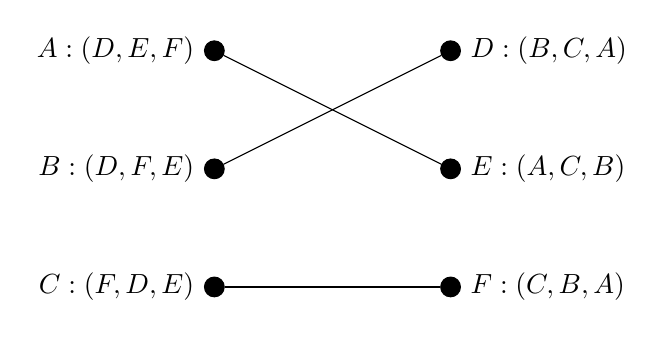
\begin{tikzpicture}[scale=0.5]

    % Suitors
    \node[draw, shape=circle, fill, inner sep=0, minimum size=0.25cm, 
    label=left: {\(A: (D, E, F)\)}] (A) at (0, 0) {};
    \node[draw, shape=circle, fill, inner sep=0, minimum size=0.25cm, 
    label=left: {\(B: (D, F, E)\)}] (B) at (0, -3) {}; 
    \node[draw, shape=circle, fill, inner sep=0, minimum size=0.25cm, 
    label=left: {\(C: (F, D, E)\)}] (C) at (0, -6) {};

    % Reviewers
    \node[draw, shape=circle, fill, inner sep=0, minimum size=0.25cm, 
    label=right: {\(D: (B, C, A)\)}] (D) at (6, 0) {};
    \node[draw, shape=circle, fill, inner sep=0, minimum size=0.25cm, 
    label=right: {\(E: (A, C, B)\)}] (E) at (6, -3) {};
    \node[draw, shape=circle, fill, inner sep=0, minimum size=0.25cm,
    label=right: {\(F: (C, B, A)\)}] (F) at (6, -6) {};

    % Lines
    \draw (A) -- (E);
    \draw (B) -- (D);
    \draw (C) -- (F);

\end{tikzpicture}
\caption{An example of a stable matching for our
    game.}\label{fig:stable_matching}

    \end{figure}
\end{example}


\balg%
    \caption{The hospital-resident algorithm
        (resident-optimal)}\label{alg:hospital_resident}
    \KwIn{a set of residents \(R\), a set of hospitals \(H\), a set of hospital
        capacities \(C\), two preference list functions \(f, g\)}
    \KwOut{a stable, resident-optimal mapping \(M\) between \(R\) and \(H\)}

    \For{\(h \in H\)}{%
        \(M^{-1}(h) \gets \emptyset\)
    }
    \While{There exists any unmatched \(r \in R\) with a non-empty preference
        list}{%
        Take any such resident \(r\) and their most preferred hospital \(h\)\;
        \(\textsc{MatchPair}(s, h)\)\;

        \If{\(\abs*{M^{-1}(h)} > c_h\)}{%
            Find their worst match \(r' \in M^{-1}(h)\)\;
            \(\textsc{UnmatchPair}(r', h)\)\;
        }
        \If{\(\abs*{M^{-1}(h)} = c_h\)}{%
            Find their worst match \(r' \in M^{-1}(h)\)\;
            \For{each successor \(s \in g(h)\) to \(r'\)}{%
                \(\textsc{DeletePair}(s, h)\)
            }
        }
    }
\ealg%

\balg%
    \caption{\textsc{MatchPair}}\label{alg:match}
    \KwIn{a resident \(r\), a hospital \(h\), a matching \(M\)}
    \KwOut{an updated matching \(M\)}

    \(M^{-1}(h) \gets M^{-1}(h) \cup \left\{r\right\}\)\;
\ealg%

\balg%
    \caption{\textsc{UnmatchPair}}\label{alg:unmatch}
    \KwIn{a resident \(r\), a hospital \(h\), a matching \(M\)}
    \KwOut{an updated matching \(M\)}

    \(M^{-1}(h) \gets M^{-1}(h) \setminus \left\{r\right\}\)\;
\ealg%

\balg%
    \caption{\textsc{DeletePair}}\label{alg:delete}
    \KwIn{a resident \(r\), a hospital \(h\)}
    \KwOut{updated preference lists}

    \(f(r) \gets f(r) \setminus \left\{h\right\}\)\;
    \(g(h) \gets g(h) \setminus \left\{r\right\}\)\;
\ealg%

\balg%
    \caption{The proposed initialisation method}\label{alg:proposed_method}
    \KwIn{a dataset \(\mathcal{X} \subset \mathcal{A}\), a number of modes to
        find \(k\)}
    \KwOut{a set of \(k\) initial modes \(\overline Z\)}

    \(\overline Z \gets \emptyset\)\;
    \(H \gets \emptyset\)\;
    \(R \gets \textsc{SamplePotentialModes}\left(\mathcal{X}\right)\)\;

    \For{\(r \in R\)}{%
        Find the set of \(k\) data points \(H_r \subset \mathcal{X}\) that 
        are the least dissimilar to \(r\)\;
        Arrange \(H_r\) into descending order of similarity with respect to
        \(r\), denoted by \(H_r^*\)\;
        \(H \gets H \cup H_r\)\;
        \(f(r) \gets H_r^*\)\;
    }

    \For{\(h \in H\)}{%
        \(c_h \gets 1\)\;
        Sort \(R\) into descending order of similarity with respect to \(h\),
        denoted by \(R^*\)\;
        \(g(h) \gets R^*\)
    }

    Solve the matching game defined by \((R, H)\) to obtain a matching \(M\)\;
    \For{\(r \in R\)}{%
        \(\overline Z \gets \overline Z \cup \left\{M(r)\right\}\)
    }
\ealg%


\section{Experimental results}\label{sec:results}

To give comparative results on the quality of the initialisation processes 
defined in
Sections~\ref{sec:init},~\ref{sec:proposed-method}~\&~\ref{sec:preferences},
four well-known, categorical, labelled datasets \- soybean, mushroom, breast
cancer, and zoo animal \- will be clustered by the \(k\)-modes algorithm with
each of the initialisation processes using their respective number of classes as
the number of clusters. These datasets have been chosen to fall in line with the
established literature, and for their relative sizes and complexities.

Typically, the quality of a clustering algorithm is measured by its performance
at classifying datasets~\cite{Huang1998}\cite{Cao2009}~\cite{Olaode2014}. In
this work, however, we will not follow this approach since our motivation is to
compare the quality of the clustering produced when using these initialisation
methods. So, for the purposes of measuring the performance of our various
initialisation methods as parts of a clustering algorithm, we will make use of
internal metrics that are independent of any external information such as a
class labelling. This family of metrics are built up from two characteristics of
the clusters found: cohesion and separation. Cluster cohesion is effectively the
summed, within-cluster variation or dissimilarity of its points, whereas a
cluster's separation is a sum of the distances between all points in the cluster
and every other point not in the cluster. In this analysis, we will make use of
two internal measures for cluster validity: our cost function from
Definition~\ref{def:cost} and the average silhouette coefficient, or silhouette
score, of our clustering, defined below. 

\begin{definition}\label{def:silhouette}
    Let \textbf{X} be a dataset and consider a clustering of \textbf{X} into
    \(k\) parts, denoted by \(C = \left\{C_1, \ldots, C_k\right\}\). For each
    \(X^{(i)} \in \textbf{X}\), we define the following two quantities:
    \begin{itemize}
        \item Let \(a\left(X^{(i)}\right)\) denote the average dissimilarity
            between \(X^{(i)}\) and every other point in its cluster. Without
            loss of generality, let \(X^{(i)} \in C_l\). Then:
            \[
                a\left(X^{(i)}\right) := \frac{1}{|C_l|} D\left(C_l,
                X^{(i)}\right)
            \]
        \item Let \(b\left(X^{(i)}\right)\) denote the lowest average 
            dissimilarity between \(X^{(i)}\) and all other points in each
            cluster other than \(C_l\). That is:
            \[
                b\left(X^{(i)}\right) := \min_{l' \neq l} \left\{
                \frac{1}{|C_{l'}|} D\left(C_{l'}, X^{(i)}\right) \right\}
            \]\\
    \end{itemize}

    With these quantities we define, for each point in our datset, their
    \emph{silhouette coefficient}, denoted by \(s(X^{(i)})\):
    \[
        s(X^{(i)}) := \frac{b\left(X^{(i)}\right) -
        a\left(X^{(i)}\right)}{\max\left\{a\left(X^{(i)}\right),
        b\left(X^{(i)}\right)\right\}}
    \]

    The \emph{silhouette score} of a clustering \(C\) is simply the average of
all the silhouette coefficients. Silhouette scores take value in the range
\([-1, 1]\). Negative scores generally suggest that elements in the data have
been mis-clustered since there exists a closer cluster centre than its own.
Values around 0 indicate overlapping clusters, whereas silhouette scores close
to 1 suggest well-separated and effective clusters.
\end{definition}


\subsection{The datasets}\label{subsec:datasets}

As stated above, the datasets being used for this work are well-known and openly
available. Below is a summary of their properties and access links for each.

\subsubsection*{Soybean}

The soybean dataset describes 35 characteristics of 307 soybean instances to
classify which disease is present. The attributes are encoded numerically as
integers but will be considered as strings for this analysis.
The diseases form .8 classes, though the first 15 are the only ones used since
they contain a considerable number of instances each~\cite{Soybean}. 
Available~at:~\url{https://archive.ics.uci.edu/ml/datasets/Soybean+(Large)}.

\subsubsection*{Mushroom}

The mushroom dataset was constructed to classify 8124 mushroom instances forming
23 species found in North America into two classes: edible and poisonous. The
attributes describe the physical characteristics and habitat of the mushrooms,
and are encoded as strings~\cite{Mushroom}. Available~at:~\url{https://archive.
ics.uci.edu/ml/datasets/mushroom}.

\subsubsection*{Breast cancer}

Wisconsin University constructed the breast cancer dataset using a decision tree
with linear programming as a diagnostic tool. The features were created using
digital images of a fine needle aspirate of a breast mass to describe the
structure of cell nuclei. There are 5.8 instances and 32 attributes in total.
Available~upon~request~to~members~of~the~academic~community~at:~\url{https://
archive.ics.uci.edu/ml/datasets/Breast+Cancer+Wisconsin+(Diagnostic)}.

\subsubsection*{Zoo animal}

The zoo animal dataset is an entirely artificial dataset used to classify 101
animals into 7 classes, those being mammal, reptile, amphibian, bird, fish,
insect, and crustacean. The 17 attributes include the name of the animal and a
series of Boolean variables describing characteristics and the habitat of the
animals. Available~at:~\url{http://archive.ics.uci.edu/ml/datasets/zoo}.

\subsection{Results}\label{subsec:results}

In this section, two sets of results will be considered. The first are the more
classically seen tables of metrics defined above, and the latter are a
collection of plots showing the descent in the cost function of the \(k\)-modes
algorithm over time. In either case, results are generated using the Python
library \href{https://github.com/nicodv/kmodes}{\texttt{kmodes}} to which the
proposed method has been added as another initialisation method. The number of
clusters to be determined, \(k\), is chosen as the number of classes associated
with each dataset. Note that this value may not be optimal (as suggested by the
relatively low silhouette scores in most cases), and that the class variable is
not considered in the running of the algorithm.

\subsubsection{Metric results}

Each of the tables of results given below were obtained by running the
\(k\)-modes algorithm 25 times with each initialisation method on the dataset in
question. For each of these 25 runs, the simulation is seeded to make the
results reproducible.

At each run of the experiment the number of epochs to termination, the initial
and final costs, and the average silhouette score were recorded for the
clustering found. These metrics are summarised below in
Tables~\ref{tab:soybean_results}~\--~\ref{tab:zoo_animal_results} by their mean
and median values, and their standard deviation over the 25 runs.

\singlespacing%
\begin{table}[H]
    \centering
    \resizebox{.9\textwidth}{!}{%
        \begin{tabular}{llrrrr}
\toprule
Initialisation & {} &  No. of iterations &  Initial cost &  Final cost &  Silhouette score \\
\midrule
Cao & mean &             2.0000 &     1574.0000 &   1314.0000 &            0.2349 \\
    & median &             2.0000 &     1574.0000 &   1314.0000 &            0.2349 \\
    & std &             0.0000 &        0.0000 &      0.0000 &            0.0000\\
\midrule
Huang & mean &             3.7600 &     1795.4400 &   1455.3200 &            0.1212 \\
    & median &             4.0000 &     1830.0000 &   1428.0000 &            0.1234 \\
    & std &             1.0520 &      131.9621 &     72.7637 &            0.0357 \\
\midrule
Matching Best & mean &             3.6800 &     1773.2400 &   1449.6400 &            0.1205 \\
    & median &             3.0000 &     1781.0000 &   1443.0000 &            0.1193 \\
    & std &             1.1075 &      118.8992 &     63.0971 &            0.0247 \\
\midrule
Matching Random & mean &             3.8800 &     1774.3600 &   1438.8000 &            0.1237 \\
    & median &             4.0000 &     1780.0000 &   1431.0000 &            0.1291 \\
    & std &             1.0924 &      121.9911 &     54.0301 &            0.0234 \\
\midrule
Matching Worst & mean &             4.0400 &     1774.9600 &   1431.8400 &            0.1290 \\
    & median &             4.0000 &     1777.0000 &   1430.0000 &            0.1291 \\
    & std &             1.0985 &      123.0411 &     53.9859 &            0.0248 \\
\midrule
Random & mean &             3.6800 &     1638.8000 &   1351.2400 &            0.1608 \\
    & median &             3.0000 &     1626.0000 &   1345.0000 &            0.1620 \\
    & std &             1.1804 &       98.2480 &     36.3126 &            0.0312 \\
\bottomrule
\end{tabular}

    }
    \captionof{table}{Summative metric results for the soybean dataset with
    \(k=15\).}\label{tab:soybean_results}\vspace{20pt}

    \resizebox{.9\textwidth}{!}{%
        \begin{tabular}{llrrrr}
\toprule
Initialisation & {} &  No. of iterations &  Initial cost &  Final cost &  Silhouette score \\
\midrule
Cao & mean &             2.0000 &    63242.0000 &  62644.0000 &            0.2517 \\
    & median &             2.0000 &    63242.0000 &  62644.0000 &            0.2517 \\
    & std &             0.0000 &        0.0000 &      0.0000 &            0.0000 \\
\midrule
Huang & mean &             2.8400 &    75107.8400 &  63231.8400 &            0.2274 \\
    & median &             3.0000 &    76026.0000 &  63002.0000 &            0.2179 \\
    & std &             0.9866 &     5864.1758 &   1059.4049 &            0.0332 \\
\midrule
Matching Best & mean &             2.8400 &    74822.2800 &  63319.5600 &            0.2209 \\
    & median &             3.0000 &    75192.0000 &  63015.0000 &            0.2179 \\
    & std &             1.0279 &     4914.2731 &   1186.2087 &            0.0345 \\
\midrule
Matching Random & mean &             2.8400 &    74822.2800 &  63319.5600 &            0.2209 \\
    & median &             3.0000 &    75192.0000 &  63015.0000 &            0.2179 \\
    & std &             1.0279 &     4914.2731 &   1186.2087 &            0.0345 \\
\midrule
Matching Worst & mean &             2.8400 &    74822.2800 &  63319.5600 &            0.2209 \\
    & median &             3.0000 &    75192.0000 &  63015.0000 &            0.2179 \\
    & std &             1.0279 &     4914.2731 &   1186.2087 &            0.0345 \\
\midrule
Random & mean &             2.6400 &    78345.8400 &  63824.8000 &            0.2243 \\
    & median &             2.0000 &    78603.0000 &  63155.0000 &            0.2281 \\
    & std &             0.8103 &     6146.4742 &   1684.9847 &            0.0391 \\
\bottomrule
\end{tabular}

    }
    \captionof{table}{Summative metric results for the mushroom dataset with
    \(k=2\).}\label{tab:mushroom_results}
\end{table}

\begin{table}[H]
    \centering
    \resizebox{.9\textwidth}{!}{%
        \begin{tabular}{llrrrr}
\toprule
Initialisation & {} &  No. of iterations &  Initial cost &  Final cost &  Silhouette score \\
\midrule
Cao & mean &             3.0000 &     3546.0000 &   3250.0000 &            0.3453 \\
    & median &             3.0000 &     3546.0000 &   3250.0000 &            0.3453 \\
    & std &             0.0000 &        0.0000 &      0.0000 &            0.0000 \\
\midrule
Huang & mean &             2.0400 &     3809.3200 &   3428.3200 &            0.1655 \\
    & median &             2.0000 &     3846.0000 &   3492.0000 &            0.0933 \\
    & std &             0.4546 &      206.2981 &    151.9832 &            0.1595 \\
\midrule
Matching Best & mean &             2.0400 &     3804.7200 &   3386.4000 &            0.1943 \\
    & median &             2.0000 &     3803.0000 &   3257.0000 &            0.3439 \\
    & std &             0.4546 &      177.0794 &    146.2635 &            0.1681 \\
\midrule
Matching Random & mean &             2.0400 &     3804.7200 &   3386.4400 &            0.1940 \\
    & median &             2.0000 &     3803.0000 &   3257.0000 &            0.3439 \\
    & std &             0.4546 &      177.0794 &    146.2247 &            0.1677 \\
\midrule
Matching Worst & mean &             2.0400 &     3804.7200 &   3386.4400 &            0.1940 \\
    & median &             2.0000 &     3803.0000 &   3257.0000 &            0.3439 \\
    & std &             0.4546 &      177.0794 &    146.2247 &            0.1677 \\
Random & mean &             2.0400 &     4150.8000 &   3349.9200 &            0.2338 \\
    & median &             2.0000 &     3682.0000 &   3250.0000 &            0.3453 \\
    & std &             0.3512 &      828.8702 &    136.8819 &            0.1631 \\
\bottomrule
\end{tabular}

    }
    \captionof{table}{Summative metric results for the breast cancer dataset
    with \(k=2\).}\label{tab:breast_cancer_results}\vspace{20pt}

    \resizebox{.9\textwidth}{!}{%
        \begin{tabular}{llrrrr}
\toprule
Initialisation & {} &  No. of iterations &  Initial cost &  Final cost &  Silhouette score \\
\midrule
Cao & mean &             2.0000 &      377.0000 &    232.0000 &            0.3860 \\
    & median &             2.0000 &      377.0000 &    232.0000 &            0.3860 \\
    & std &             0.0000 &        0.0000 &      0.0000 &            0.0000 \\
\midrule
Huang & mean &             2.4800 &      360.2800 &    250.3200 &            0.3047 \\
    & median &             2.0000 &      358.0000 &    244.0000 &            0.3271 \\
    & std &             0.6532 &       41.1213 &     15.2226 &            0.1038 \\
\midrule
Matching Best & mean &             2.3600 &      359.6800 &    251.8400 &            0.3045 \\
    & median &             2.0000 &      352.0000 &    252.0000 &            0.3184 \\
    & std &             0.4899 &       42.6602 &     12.5322 &            0.0926 \\
\midrule
Matching Random & mean &             2.4000 &      360.5200 &    252.6000 &            0.3083 \\
    & median &             2.0000 &      352.0000 &    253.0000 &            0.3300 \\
    & std &             0.5000 &       42.5853 &     12.1587 &            0.0938 \\
\midrule
Matching Worst & mean &             2.4800 &      367.0000 &    249.8800 &            0.3047 \\
    & median &             2.0000 &      356.0000 &    252.0000 &            0.3138 \\
    & std &             0.6532 &       42.7444 &      9.8375 &            0.0729 \\
\midrule
Random & mean &             2.4000 &      340.0800 &    265.2000 &            0.2658 \\
    & median &             2.0000 &      335.0000 &    253.0000 &            0.3122 \\
    & std &             0.7638 &       58.5227 &     27.1953 &            0.1204 \\
\bottomrule
\end{tabular}

    }
    \captionof{table}{Summative metric results for the zoo animal dataset with
    \(k=7\).}\label{tab:zoo_animal_results}
\end{table}
\doublespacing%

\subsubsection{Epoch costs}

The epoch-cost plots in this section were created by setting an initial seed for
each initialisation method and then running the \(k\)-modes algorithm 25 times.
Of these runs, the best set of costs is then chosen by their final cost and
plotted.

Note that in each figure, dotted lines indicate the established initialisation
methods whilst solid lines are used for the proposed method.

\begin{figure}[h!]
    \centering
    \includegraphics[width=.8\textwidth]{./img/epoch_plot_soybean.pdf}
\end{figure}

\begin{figure}[h!]
    \centering
    \includegraphics[width=.8\textwidth]{./img/epoch_plot_mushroom.pdf}
\end{figure}

\begin{figure}[h!]
    \centering
    \includegraphics[width=.8\textwidth]{./img/epoch_plot_breast_cancer.pdf}
\end{figure}

\begin{figure}[h!]
    \centering
    \includegraphics[width=.8\textwidth]{./img/epoch_plot_zoo_animal.pdf}
\end{figure}

\section{Conclusion}\label{sec:conclusion}

In this paper a novel initialisation method for the \(k\)-modes was introduced
that built on the method set out in the seminal paper~\cite{Huang1998}. The new
method models the final `replacement' process in the original as an instance of
the Hospital-Resident Assignment Problem that may be solved to be mathematically
fair and stable.

Following a thorough description of the \(k\)-modes algorithm and the
established initialisation methods, a comparative analysis was conducted amongst
the three initialisations using both benchmark and artificial datasets. This
analysis revealed that the proposed initialisation was able to outperform both
of the other methods when the choice of \(k\) was optimised according to a
mathematically rigorous elbow method. However, the proposed method was unable to
beat Cao's method (established in~\cite{Cao2009}) when an external framework was
imposed on each dataset by choosing \(k\) to be the number of classes present.

The proposed method should be employed over Cao's when there are no hard
restrictions on what \(k\) may be, or if there is no immediate evidence that the
dataset at hand has some notion of high density. Otherwise, Cao's method remains
the most reliable initialisation in terms of computational time and final cost.


\bibliography{references}

\end{document}
